\documentclass[crop, tikz]{standalone}

\usepackage[utf8]{inputenc}
% 'crop' is the default for v1.0, before it was 'preview'
%\usetikzlibrary{...}% tikz package already loaded by 'tikz' option

\usetikzlibrary{arrows}
\usetikzlibrary{decorations.markings}
\usetikzlibrary{patterns}
\usetikzlibrary{calc}

%hexagon drawing variables
\def\ly{0.866025} %sin(pi/3) = sqrt(3)/2
\def\lx{0.5} %cos(pi/3) = 0.5
\def\hexSize{5} %size of the hexagon that'll be the extent of the fibre cross section
\def\coreSize{0.2} %size of hollow cores
\def\coreSep{0.5} %separation between core CENTRES HORIZONTALLY
\def\coreSepHeight{0.4464} %separation between core CENTRES VERTICALLY

\newcommand{\hexagon}[4]{
\begin{scope}[shift={#2}]
	\draw[#3, fill=#4] (-#1*\lx, #1*\ly) -- (#1*\lx, #1*\ly) -- (#1,0) -- (#1*\lx, -#1*\ly) -- (-#1*\lx, -#1*\ly) -- (-#1,0) -- cycle;
\end{scope}
} %\hexagon{centre-to-corner-length}{shift (x,y)}{line spec}{fill colour} [none is allowed for fillcolour]

\begin{document}
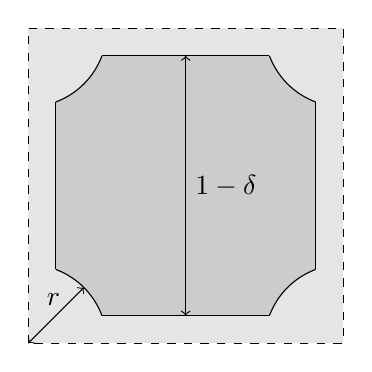
\begin{tikzpicture}[]

	% drawing acrs of circles
	\def\centreArc[#1](#2)(#3:#4:#5)% Syntax: [draw options] (center) (initial angle:final angle:radius)
    { \draw[#1] ($(#2)+({#5*cos(#3)},{#5*sin(#3)})$) arc (#3:#4:#5); }
	% define some sizes to draw consistently
	\def\l{0.35}
	\def\rectSize{4}
	\def\r{\rectSize*0.25}
	\def\alpha{asin(\l/(\r)}
	% colours
	\def\inc{black!20!white}
	\def\bulk{black!10!white}

	% inclusion colour, to overwrite momentarily
	\fill[\inc, draw=black, dashed] (0,0) rectangle (\rectSize,\rectSize);
	% now fill in the "background" using cunning shapes
	\fill[\bulk] (0,0) rectangle (\rectSize,\l);
	\fill[\bulk] (0,0) rectangle (\l,\rectSize);
	\fill[\bulk] (0,\rectSize) rectangle (\rectSize,\rectSize-\l);
	\fill[\bulk] (\rectSize,0) rectangle (\rectSize-\l,\rectSize);
	\fill[\bulk] (\r,0) arc [start angle=0,end angle=90,x radius=\r,y radius=\r] -- (0,0) -- cycle;
	\fill[\bulk] (0,\rectSize-\r) arc [start angle=270,end angle=360,x radius=\r,y radius=\r] -- (0,\rectSize) -- cycle;
	\fill[\bulk] (\rectSize-\r,\rectSize) arc [start angle=180,end angle=270,x radius=\r,y radius=\r] -- (\rectSize,\rectSize) -- cycle;
	\fill[\bulk] (\rectSize,\r) arc [start angle=90,end angle=180,x radius=\r,y radius=\r] -- (\rectSize,0) -- cycle;
	%draw dotted period cell outline now to avoid overwrite errors
	\draw[dashed] (0,0) rectangle (\rectSize,\rectSize);

	% now draw the inclusion in such a way as to emphasise the vertex volume
	% BLL to BRL
	\draw ({sqrt(\r*\r - \l*\l)},\l) -- ({\rectSize-sqrt(\r*\r - \l*\l)},\l);
	% BRL to BRU
	\centreArc[black](\rectSize,0)(180-\alpha:90+\alpha:\r)
	% BRU to TRL
	\draw (\rectSize-\l,{sqrt(\r*\r - \l*\l)}) -- (\rectSize-\l,{\rectSize-sqrt(\r*\r - \l*\l)});
	% TRL to TRU
	\centreArc[black](\rectSize,\rectSize)(270-\alpha:180+\alpha:\r)
	% TRU to TLU
	\draw ({sqrt(\r*\r - \l*\l)},\rectSize-\l) -- ({\rectSize-sqrt(\r*\r - \l*\l)},\rectSize-\l);
	% TLU to TLL
	\centreArc[black](0,\rectSize)(360-\alpha:270+\alpha:\r)
	% TLL to BLU
	\draw (\l,{sqrt(\r*\r - \l*\l)}) -- (\l,{\rectSize-sqrt(\r*\r - \l*\l)});
	% BLU to BLL
	\centreArc[black](0,0)(90-\alpha:\alpha:\r)

	% annotating arrows for length scales?
	\draw[<->] (0,0) -- ({\r/sqrt(2)},{\r/sqrt(2)}); 
	\node[anchor=south east] at ({0.75*\r/sqrt(2)},{0.5*\r/sqrt(2)}) {$r$};
	\draw[<->] (\rectSize/2,\l) -- (\rectSize/2,\rectSize-\l);
	\node[anchor=west] at (\rectSize/2,\rectSize/2) {$1-\delta$};

\end{tikzpicture}
\end{document}